\chapter{The Lorentz transformation}

\newpage
\thispagestyle{empty}

\begin{figure}[H]
\centering
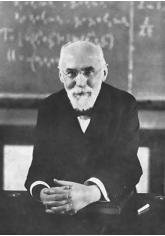
\includegraphics[scale=1]{src/images/lbk-graphics/portraits/Lorentz.pdf}
\caption*{Hendrik Antoon Lorentz}
\end{figure}
%~ \portrait{2}{lbk-graphics/portraits/Lorentz.pdf}%
%~ {Hendrik Antoon Lorentz}
\begin{small}
\begin{quote}

Hendrik Antoon Lorentz (18 July 1853--4 February 1928) was a 
Dutch physicist who shared the 1902 Nobel Prize in Physics 
with Pieter Zeeman for the discovery and theoretical 
explanation of the Zeeman effect. He also derived the 
transformation equations which formed the basis of the 
special relativity theory of Albert Einstein.
\end{quote}

\begin{quote}
``It may well be said that Lorentz was regarded by all 
theoretical physicists as the world's leading spirit, who 
completed what was left unfinished by his predecessors and 
prepared the ground for the fruitful reception of the new 
ideas based on the quantum theory.'' --From the biography 
published by the Nobel Foundation: \dm \hfill --Wikipaedia
\end{quote}

\newpage

\section{Introduction}
In Chapter~1, we noted how one may transform the 
absolute frame of Newton and realise an infinite class of 
reference frames, called Galilei frames, in each one of 
which the Newton laws of motion hold equally well. This 
clearly implied that the Newton laws of motion would not 
serve to identify the absolute frame from among the class 
of all Galilei frames. One had to look for other possible 
methods of identifying the absolute frame. Precisely such a 
method was suggested by Maxwell based on his electromagnetic 
theory: Maxwell's suggested that the Newtonian absolute 
frame is the unique Galilei frame relative to which light 
propagates isotropically in ether. Notable among the 
experiments done to test this idea were those of Michelson 
and Morley (see chapter~2) which decisively failed to detect 
any anisotropy in the prospagation of light in a moving 
Galilei frame. One could not understand this (experimentally 
revealed) behaviour of light which clearly seemed to defy 
the Galilei transformation.

\hsl{Lorentz frames}
In his 1905 paper\footnote{A. Einstein, \textsl{Zur 
Electrodynamic bewegter Korper}, Ann. Phys., Leipzig, 
\textbf{17}, 891, 1905},  Albert Einstein came up with a 
solution to this puzzle posed by the behaviour of light. 
\begin{quote}
\textsl{He introduced the postulate that there exist special 
coordinate systems, called \textsl{Lorentz 
frames}\footnote{According to the general theory of 
relativity, is impossible to construct global Lorentz 
frames, \ie, pseudo-Cartesian space-time coordinate systems 
covering the whole of spacetime, when gravitational fields 
are present. As such, when dealing with physical phenomena 
involving the gravitational field, if needed, one 
necessarily has to consider \textsl{local} Lorentz frames 
only. Such a local Lorentz frame is a spacetime coordinate 
system defined in the neighbourhood of an event of interest 
$P$, and its Lorentz nature is restricted only to a 
sufficiently small region of spacetime around $P$. However, 
in special relativity theory, which does not include the 
phenomenon of gravitation, global Lorentz frames, which are 
described in the following section, are certainly 
admissible. Later, in Appendix 6B (\S~6.20), we identify a 
Lorentz frame as a true inertial frame in which the Maxwell 
equations in vacuum and the first law of Newton, are both 
valid. A Galilei frame would then be seen as a frame which 
is only approximately inertial in the Newtonian limit.}, 
relative to each one of which light propagates in vacuum 
with the same speed in all spatial directions}.
\end{quote}
This postulate is called \textsl{the principle of constancy 
of the speed of light}. The null result of the 
Michelson-Morley experiment would then be a natural 
consequence of this principle once we treat both the frames 
of reference in the experiment, namely the earth-bound 
frame 
of the interferometer, and the \textsl{absolute frame} in 
which ether is supposed to be at rest, as Lorentz frames.

The principle of the constancy of light clearly  required 
that a transformation relating two Lorentz frames must be a 
symmetry transformation of the Maxwell equations. 
``\textsl{Early approximations of $\cdots$[such a] 
transformation were published by Voigt (1887) and Lorentz 
(1895). They were completed by Larmor (1897, 1900) and 
Lorentz (1899, 1904) and were brought into their modern 
form by Poincare (1905), who gave the transformation the 
name of Lorentz.{}}''{}{}\footnote{History of Lorentz 
transformations--IPFS, https://ipfs.io/ipfs/.../wiki/
History\_of\_Lorentz\_transformations.html}

\begin{quote}
\textsl{Einstein in his 1905 paper introduced a second 
postulate\footnote{The first postulate is the principle 
of constancy of the speed of light.} called  \textbf{the 
principle of relativity} to his theory.  The 
principle of relativity required\footnote{See the quotation 
from Niel Russell 
in CERN COURIER given at the beginning of \S~4.1} that  all 
laws of physics (except the laws of gravity) possess 
\textsl{Lorentz symmetry}.  In the same paper, Einstein 
showed that the Lorentz transformation follows from the 
principles of relativity and that of the constancy of the 
speed of light.}
\end{quote}
A detailed discussion of the Lorentz transformation is 
presented in \S~4.3; Immediately, in the following section 
\S4.2, we briefly discuss a few basic concepts.

\vspace{-.2cm}

\section{Minkowski spacetime}
\hsl{Point-event} A point-event $P$ occurs at a definite 
spatial location and at a definite instant of 
time. As an example of a point-event, we may mention the 
collision of two mass-points. The spatial location and the 
time-instant of occurance together constitute a 
\textbf{spacetime point}. In relativity theory, it is 
customary to refer to a spacetime point $P$ also as the 
``event'' $P$. The totality of all spacetime points, or 
events, constitutes \textsl{spacetime}. 

\hsl{Minkowski spacetime} The spacetime of the special 
relativity theory, called the \textsl{Minkowski spacetime}, 
is a four dimensional mathematical space $\mathbb{M}$. 
Points of $\mathbb{M}$ are called \textsl{events}. 
$\mathbb{M}$ is assumed to be a \textsl{4-dimensional, flat, 
Riemannian  manifold}  which may be \textsl{coordinatized} 
by a single \textsl{global} coordinate system called a 
\textsl{pseudo-Cartesian coordinate system}. 

\hsl{Lorentz frame}A pseudo-Cartesian coordinate system 
which covers the whole of $\mathbb{M}$, is also called  a 
\textsl{Lorentz frame}.  

\newpage

Relative to a Lorentz frame, every event $P\in \mathbb{M}$ 
is associated with a real quadtuplet of coordinates  
$(ct,\;x,y,z)$ where 
\begin{align*} 
-\infty<ct<\infty,   \quad -\infty< x, y, z<\infty,   
\end{align*} 
and $c$ is the speed of light in vacuum. observe that using 
$ct$ instead of the coordinate  $t$  makes all the four 
coordinates $ct$, $x$, $y$ and $z$ of the event $P$ to have 
the same physical dimension of a length\footnote{It is a 
matter of taste to have the dimension of a length for all 
the four coordinates of an event. One could have chosen all 
the four coordinates to have the dimension of time. Some 
times, one conveniently works in units called 
\textsl{natural units} in which $ct$ and 
$t$ have the same dimension because one would set  $c = 1$ 
.}. 

\subsection{Point-objects}

\hsl{Material particle} A material particle 
\index{material particle} \index{mass-point} or 
mass-point\footnote{A point-object is called a 
\textsl{tardyon}, \index{tardyon} a l\textsl{uxon } 
\index{luxon} or a \textsl{tachyon} \index{tachyon} 
according as its speed is \textsl{slower}, 
\textsl{equal to}, or \textsl{faster than} that of 
light in vacuum. Note that a tachyon is, to date, only 
an \textsl{interesting concept}: No body has ever 
observed a tachyon so far.}, is a geometrical point in 
space endowed with a non-zero mass\footnote{A mass-point 
is conveniently labelled by its invariant-mass or its  
rest-mass (cf. \S6.13) }. In every Lorentz frame, 
a material particle moves with a speed \textsl{less than} 
$c$. 

\hsl{Charged particle}A charged particle is a material 
particle endowed with a non-zero electric charge. 
\index{charged particle}

\hsl{Light corpuscle} A light corpuscle, also called a 
\textsl{luxon}, is a point-object which always moves 
with the speed $c$ in every Lorentz frame. \index{light 
corpuscle}

\subsection{World lines}
\index{world lines} 
In a Lorentz frame $S$, consider a point-object 
\index{point-object} $P$ (which can be a material 
particle or a luxon) moving on a space orbit described 
by the parametric equation $\vec{r}=\vec{r}(t)$. At a 
given instant of time $t$, the three space coordinates 
$x(t),y(t), z(t)$ of the point-object and $w\equiv ct$ 
together define the {event} $(w(t)\equiv ct, x(t), 
y(t), z(t))$. As time evolves, say, in some domain $t_1 
\leq t\leq t_2$, the moving point-object similarly gets 
associated with a continuous set of events $\{(w(t), 
x(t),y(t), z(t))\}$. To keep things general, in 
the place of $t$, one could introduce a new parameter 
$\gkl\equiv \gkl(t)$, which is an arbitrary continuous 
function of  $t$ in the domain $t_1 \leq t\leq t_2$, 
and re-express the elements of this  continuous set of 
events  $\{(w(t), x(t),y(t), z(t))\}$ as 
$\{x^0(\gkl)\equiv w[t(\gkl)] $, \; $x^1(\gkl) \equiv 
x[t(\gkl)] $, \;$x^2(\gkl)\equiv 
y[t(\gkl)]$,\;$x^3(\gkl)\equiv z[t(\gkl)]$\}.

Now, imagine a parametric ``plot'' of the events belonging 
to the set $\{x^\gka(\gkl),\;\gka=0,1,2,3 \}$ against 
$\gkl$: Such a ``plot''  would then be a curve in $\mbb{M}$ 
with the parametric equation $x^\gka=x^\gka(\gkl)$.

\dfn The locus  of all events associated with a 
point-object 
$P$ is a parametrized curve $x^\gka =x^\gka(\gkl)$ 
in $\mathbb{M}$ called its \textsl{world line} or 
\textsl{history}. \index{history of a point-object} 

\hsl{A point-object at  rest} It is also useful to note 
that if the point object is at \textsl{rest} at the space 
point $P$ in the Lorentz frame $S$, and consequently has 
three constant space coordinates, say 
$x_\sfx{P},y_\sfx{P},z_\sfx{P}$, then,  as before, one may 
define the continuum of events $\{x^0(\gkl), 
x^1(\gkl)=x_\sfx{P}, x^2(\gkl)=y_\sfx{P}, 
x^3(\gkl)=z_\sfx{P}\}$  where the \textsl{same} triple of 
spatial coordinates $x_\sfx{P}, y_\sfx{P},z_\sfx{P}$ are 
respectively associated with $x^1, x^2$ and $x^3$ at all 
instants $t$ in the domain $t_1 \leq t\leq t_2$. Thus, the  
world line, or history of a point-object at rest at the 
spatial point $x_\sfx{P},y_\sfx{P},z_\sfx{P}$ in the 
pseudo-Cartesian coordinate system $S$ would be a curve in 
spacetime on which the space coordinates have the constant 
values $x^1=x_\sfx{P}, x^2=y_\sfx{P}, x^3=z_\sfx{P}$.

In passing, it may be worth repeating that every 
point-object, wheth-\break er moving or not relative to a given 
Lorentz frame, is associated with a definite world line.

\subsection{Spacetime diagrams}

A schematic diagram representing a region of spacetime on a 
two-dimen\break sional Euclidean plane (such as a sheet of paper) 
is called a spacetime diagram. Such a diagram consists of 
the graphical representations of spacetime events, 
world-lines and world-surfaces on the two-dimension\break al 
Euclidean plane mentioned.

Occasionally, we make use of spacetime diagrams.  For more 
interesting material on spacetime diagrams, we refer the 
reader to the books by Synge and Burke cited at the 
beginning of this chapter.

\subsection{Measurement of time intervals: 
Standard\\ clocks} \index{ideal standard clock} 
We make time measurements using \textsl{ideal standard  
clocks}. Conceptualised, a standard clock is a 
material-point endowed with an ideal ``clock-work 
mechanism''. Being a material-point (cf. \S~4.2.1), the 
spatial location of a standard clock may be specified by a 
triplet $(x,y,z)$ of spatial-coordinates and it moves with 
a 
speed less than $c$ in every Lorentz frame.

\newpage

%\begin{wrapfigure}[13]{1}{40mm}
\begin{figure}[H]
\centering
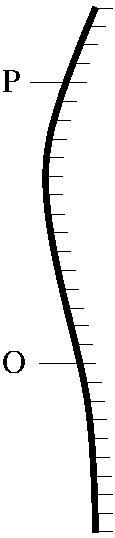
\includegraphics[scale=.5]{src/images/lbk-graphics/str5.pdf}
\caption*{}
\end{figure}
%~ \fig{.3}{lbk-graphics/str5.pdf}{}{}
%\end{wrapfigure}

The assumed ideal nature of a standard clock\footnote{Since 
we always consider standard clocks only, we shall refer to 
them simply as clocks hereafter.} implies the following: If 
$O$ is an arbitrarily chosen event on the world-line $L$ of 
the standard clock and $P$ any other later event on $L$, 
the 
number $\tau$ of clock-ticks that occur between $O$ and $P$ 
is always the same irrespective of the state of motion of 
the clock or of the external forces acting on the clock. 
The 
number $\tau$ (of clock-ticks) is taken as the time of 
occurrence of the event $P$ relative to the 
\textsl{time-origin} $O$ and is called the 
\textsl{proper-time} of $P$ relative to $O$ on $L$. This 
way, all events on $L$ may be labelled by their respective 
proper-times relative to $O$. 
\subsection{Clock synchronisation}
In \figref{fig4.2}, we show the worldlines of two clocks $A$ 
and $B$ at rest\footnote{An operational  definition of 
`being mutually at rest' is as follows: If there is no 
Doppler shift (discussed in \S~8.8 later) of the frequency 
of light signals sent form one clock to another, then they 
are at rest relative to each other} relative to each other. 
These two clocks  may be \textsl{synchronised} by using the 
so-called \textsl{radar method}: A light signal (called a 
radar signal) sent from the clock $A$ to the clock $B$ is 
reflected back to $A$. Let $t_1$ and $t_2$ be the departure 
and arrival times of the radar signal as recorded by $A$. To 
synchronise the clock $B$ with $A$, one need only set the 
clock $B$ to read  $(t_1 + t_2)/2$ at the instant $B$ 
receives the radar signal sent from $A$.

\newpage

\begin{figure}[H]
\begin{center}
\begin{tikzpicture}
% \draw[help lines,step=.25,lightgray] (-4,-4) grid (4,4) ;
%   \foreach \y in {-4,-3.5,...,4}
%   \draw (-4.25,\y) node[left]{\tiny\y} ;
%   \foreach \x in {-4,-3.5,...,5}
%   \draw (\x,-4.2) node[below]{\tiny\x} ;
\node at (0,0)%
{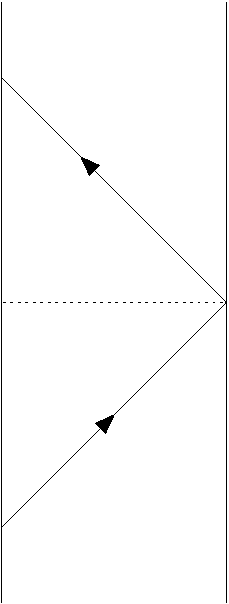
\includegraphics[scale=.5]{%
src/images/lbk-graphics/clock.pdf}};
\node at (-1,-2.75) [below]{\small  $A$} ;
\node at (1,-2.75) [below]{\small $B$} ;
\node at (-1.2,-1.8) [below]{\small $t_1$};
\node at (-1.2,1.9){\small  $t_2$};
\node at (1.8,0){\small $(t_1+t_2)/2$};
\end{tikzpicture}
\caption{}\label{fig4.2}
\end{center}
\end{figure}

\subsection{Measurement of spatial distances} 
Distances are also measured using the \textsl{radar 
method}: 
A light signal sent from the spatial point  $A$ to the 
spatial point $B$ is reflected back to $A$. If  $t_1$ and 
$t_2$ are the departure and arrival times of the radar 
signal according to a clock at rest at $A$, the spatial 
distance $\ell_{AB}$ between $A$ and $B$ is, 
\begin{align}\label{str.1}
\ell_{AB}=c(t_2-t_1)/2.
\end{align}

Using the methods of Euclidean geometry and the radar 
technique of distance measurement, one can determine the 
distances of a given spatial point $P$ from a fixed spatial 
point called the origin along the (three mutually 
perpendicular) coordinate axes which give the (Cartesian) 
spatial coordinates of $P$. By repeating this procedure, 
one 
may, \textsl{in principle}, establish a global 
pseudo-Cartesian coordinate system \ie, a Lorentz frame, in 
the whole of Minkowski spacetime.

\section{The Poincare and Lorentz\\ transformations}
\begin{quote}
\textsl{Today there is no need to justify the Poincare 
group 
as there was in Einstein's time, nor to derive it from a 
minimal set of hypotheses. Rather we  simply assert that 
the 
Poincare group is the symmetry group (at least to a high 
degree of approximation) of all physical systems and then 
explore the consequences of such an assertion. The 
justification for this assertion will then rest on the 
degree to which these consequences are borne out in 
nature.}\\ 
\dm \hfill -- J. L. Anderson in his book, \textsl{loc.cit}.
\end{quote}  

In \S~4.2, we mentioned that the Minkowski spacetime 
$\mathbb{M}$, by its (defined) nature, may be coordinatized 
using a single global Lorentz frame. However, such a 
Lorentz frame in $\mathbb{M}$ is not unique: We shall see 
that a new Lorentz frame can always be introduced in 
$\mathbb{M}$ through what is called a  \textsl{Lorentz 
transformation},  that too in many different ways. In the 
following paragraphs, we discuss a Lorentz transformation. 
To this end, we may recall the following 
\textsl{Einsteinian 
definition} of a Lorentz frame from \S~4.1: 

\dfn A Lorentz frame is a global pseudo-Cartesian 
coordinate system $S$ in $\mathbb{M}$ relative to which 
light propagates isotropically in vacuum  with the speed 
$c\sim \num{3e8}\si{m/s}$. 

The special theory of relativity is founded on the 
following 
two postulates: 

\hsl{The principle of relativity} The laws of physics (in 
the absence of gravity) are the same in all Lorentz frames. 

\hsl{The principle of constancy of the speed of light}The 
numerical value $c \sim \num{3e8}\si{m/s}$ of the speed of 
light in vacuum  is the same in all Lorentz frames. In a 
given Lorentz frame, the speed of light is the same in all 
spatial directions. 

Now, we derive\footnote{See the remarks by J. L. Anderson 
quoted at the beginning of this sectrion 4.3.} the 
coordinate transformation, called a \textsl{Poincare 
transformation}, that maps one Lorentz frame into another. 
Let\break $S: \{ x^0,x^1,x^2,x^3\}$ and  ${S}': \{x^\notp, 
x^\onep,  x^\twop,x^\trip\}$ be two Lorentz frames related 
to each 
other by the coordinate  transformation
\begin{align}\label{str.2}
x^{\gkmp} = x^{\gkmp} ( x^0,\;x^1,\;x^2,\;x^3 )\;.
\end{align}
We demand that such a coordinate transformation must    
meet the following requirements:
\begin{description}
\item [L1.] {Preserve the Euclidean nature of the 
spatial  geometry}.
\item [L2.] {Transform free particles into a free
particles}.
\item [L3.] {Preserve the fact that, in vacuum, light 
propagates in all spatial directions with the same speed  
$c$}.
\end{description}

To explore how the requirement L2 conditions the  
transformation connecting two Lorentz frames, we consider 
the following equation to the orbit of a free particle $P$ 
in a Lorentz frame $S$: 
\begin{align}\label{str.3}
\vec{r}(t) = \vec{u}\, t + \vec{r}_{\nt 0}.
\end{align}
Here, $\vec{r}(t)=x^1\,\eye+ x^2\,\jay+x^3\,\kay$ and 
$\vec{r}_{\nt 0}$ are  the position vectors of $P$ at the 
instants $t$ and $t=0$ in  $S$. 

On taking the dot-product of Eqn.\eqref{str.3} with an 
\textsl{arbitrary} constant vector $\vec{A}\,= 
(A_1\,\eye + A_2\,\jay + A_3\,\kay)$, we obtain the 
equation  $\vec{A}\, \dotp \vec{r} =(\vec{A}\,\dotp 
\vec{u}) \,t + (\vec{A}\, \dotp \vec{r}_{\nt 0})$, 
which may be rearranged as
\begin{align*}
A_0x^0+A_1x^1+A_2x^2+A_3x^3=B,
\end{align*}
or, what is the same thing, 
\begin{align}\label{str.4}
A_\gkm x^\gkm =B,
\end{align} 
where  $A_0 \equiv - (\vec{A}\,\dotp \vec{u})/c$, $B\equiv 
(\vec{A}\, \dotp \vec{r}_{0})$ and we have used the standard
\textsl{summation convention} according to which the 
\textsl{repeated, or, dummy index} $\gkm$ is to be 
summed over from $0$ to $3$. Thus, the requirement L2 
implies that the orbit of a free-particle must be given by 
an equation of the form \eqref{str.4} in every Lorentz 
frame. Since L2 must must be true of every 
free-particle-orbit, we demand that the coordinate 
transformation \eqref{str.2} must map \textsl{every} linear 
equation of the form \eqref{str.4} in the Lorentz frame 
$S$, into a corresponding linear equation
\begin{align}\label{str.5}
{A}_{\gkm'} x^{\gkm'} = {B}',
\end{align}
in the Lorentz frame $S'$ with some suitable constants 
${A}_{\gkm'}$ and $B'$. 

To proceed further, we differentiate Eqn.\eqref{str.4} and
obtain the equation  $?A_\gkm? ?{dx}^\gkm?=0$ which may 
also be expressed as 
\begin{align}\label{str.6}
?A_\gkm? ?{dx}^\gkm? 
={A}_{\gkm}?{K}^\gkm_\gknp?\,?{dx}^\gknp? = 
0, \text{ where} 
\end{align}
\begin{align}\label{str.7}
?K^\gkm_\gknp?\equiv \pdx{\gkm}{\gknp},
\end{align}
is the $\gkm\gknp$-th element of the Jacobian matrix of the
inverse coordinate transformation
\begin{align*}
x^\gka =x^\gka (x^\notp,x^\onep,x^\twop,x^\trip),
\end{align*}
associated with \eqref{str.2}. 

Now, we observe that Eqn.\eqref{str.6} must be the same as 
the equation 
\begin{align}\label{str.8}
A_{\gkn'}dx^{\gkn'} =0, 
\end{align}
which is obtained by taking the differential of 
Eqn.\eqref{str.5}. Therefore, on equating Eqn.\eqref{str.8} 
with Eqn.\eqref{str.6} and rearranging, we get, 
\begin{align}\label{str.9} 
(A_\gkm\mtud{{K}}{\gkm}{\gknp}- 
A_{\gknp}) dx^{\gknp}=0 . 
\end{align} 
Finally, since the $dx^{\gknp}$ are \textsl{arbitrary}, the 
above equation would be true only if
\begin{align}\label{str.10}
A_{\gknp}= \mtud{K}{\gkm}{\gknp}{A}_\gkm.
\end{align}
Note that this equation should convert four arbitrarily 
assignable \textbf{constants} $A_\gkm$ into four (new) 
\textbf{constants} $A_{\gknp}$ and that is possible 
\textsl{if, and only if, }\textbf{every one of the 
coefficients $?K^\gkm_{\gknp}?$ is itself a constant}. 
This, 
in turn, requires that all the elements $?L^\gkm_{\gknp}? 
\equiv(\dow {x}^\gkm /\dow x^{\gknp})$ of the forward 
Jacobian matrix (which is the inverse of the matrix 
$?{K}^\gkm_{\gknp}?$) are also constants. Armed with this 
information, we now integrate the differential of the 
equation \eqref{str.2}, namely,
\begin{align}\label{str.11}
dx^{\gkmp} = \mtud{L}{\gkmp}{\gkn}\,dx^\gkn ,
\end{align}
and obtain the finite form of the Poincare transformation 
connecting two Lorentz frames:
\begin{align}\label{str.12}
x^{\gkmp} =\mtud{L}{\gkmp}{\gkn}x^\gkn + M^{\gkmp}.
\end{align}
where, $M^{\gkmp}$ are four constants of integration. In 
geometry, transformations of the type \eqref{str.12}, are 
called \textsl{affine transformations}.

\hsl{Lorentz matrix} The sixteen constant coefficients 
$\mtud{L}{\gkmp}{\gkn} $ in the Poincare transformation 
\eqref{str.12} may be arranged into a square matrix
\begin{align}\label{str.13}
L \equiv\begin{pmatrix}
?L^{0'}_0?& ?L^{0'}_1?& ?L^{0'}_2? & ?L^{0'}_3?\\
?L^{1'}_0?& ?L^{1'}_1?& ?L^{1'}_2? & ?L^{1'}_3?\\
?L^{2'}_0?& ?L^{2'}_1?& ?L^{2'}_2? & ?L^{2'}_3?\\
?L^{3'}_0?& ?L^{3'}_1?& ?L^{3'}_2? & ?L^{3'}_3?\\
\end{pmatrix} ,
\end{align}
called a \textsl{Lorentz matrix}. In terms of the Lorentz 
matrtix $L$, we may express the Poincare transformation 
\eqref{str.12} as the matrix equation 
\begin{align}\label{str.14}
 X'=LX +M,
\end{align}
where 
\begin{align}\label{str.15}
X\equiv\begin{pmatrix}x^0\\x^1\\x^2\\x^3\end{pmatrix},
\quad 
X'\equiv\begin{pmatrix}x^{0'}\\x^{1'}\\x^{2'}\\x^{3'}   
\end{pmatrix} \text{ and }
M\equiv\begin{pmatrix}M^{0'}\\M^{1'}\\M^{2'}\\M^{3'}    
\end{pmatrix}.
\end{align}

\hsl{Homogeneous Lorentz transformation} When all the four  
constants $M^{\gkmp}$ in the Poincare  transformation 
\eqref{str.12} are zeros, we get the transformation
\begin{align}\label{str.16}
x^{\gkmp} =\mtud{L}{\gkmp}{\gkn}x^\gkn,
\end{align} 
called a \textsl{homogeneous Lorentz transformation} which 
may also be expressed as the matrix equation
\begin{align}\label{str.17}
X'=LX.
\end{align}  

\exm Prove that the affine transformation \eqref{str.12} 
maps uniform 3-velocities into uniform 3-velocities. 

\soln The $i$-th component, $i=1,2,3 $, of the 3-velocity 
of a point-object in the ``dashed-frame'' is given by
\begin{align*}
\frac{u^{i'}}{c}&\equiv \frac{dx^{i'}}{dx^{0'}} =
\frac{\mtud{L}{i'}{j} dx^j}{\mtud{L}{0'}{j} dx^j}
\\&=\frac{\mtud{L}{i'}{0} + \mtud{L}{i'}{j}(dx^j/ dx^0)}
{\mtud{L}{0'}{0} + \mtud{L}{0'}{j}(dx^j/dx^0)}
=\frac{\mtud{L}{i'}{0} + \mtud{L}{i'}{j}(u^j /c)}
{\mtud{L}{0'}{0}+\mtud{L}{0'}{j}(u^j /c) }\;.
\end{align*}
Since the $\mtud{L}{\gkmp}{\gkn}$ are all constants, this 
equation shows that  a constant\break \mbox{3-velocity} $(u^1,\; 
u^2,\;u^3)$ is mapped into a corresponding constant 
\break 3-velocity $(u^{1'},\; u^{2'},\; u^{3'})$.
\ebx

Next, we further determine the affine transformation 
\eqref{str.12} by requiring it to satisfy the condition L2. 
To this end, we consider a light corpuscle in motion in a 
Lorentz frame $S$. Recall that the spatial geometry is 
Euclidean in every Lorentz frame $\{x^\gka \}$ and as such, 
the spatial separation between two infinitesimally 
separated 
spatial points in $\{x^\gka \}$ is given by $dl^2 = 
(dx^1)^2 
+ (dx^2)^2 + (dx^3)^2 $. If the light corpuscle leaves the 
spatial point $\vec{r}_1=x_1\eye +y_1\jay +z_1\kay$ at the 
time $t_1 $ and arrives at the spatial point  $\vec{r}_2 = 
x_2 \eye +y_2 \jay +z_2\kay$ at the time $t_2$, we must have
\begin{align*}
c^2(t_2-t_1)^2&=(\vec{r}_2-\vec{r}_1)^2\notag\\
&=(x_2-x_1)^2 + (y_2-y_1)^2 + (z_2-z_1)^2,
\end{align*}
which may also be written as
\begin{align}\label{str.18}
&c^2(t_2-t_1)^2-(x_2-x_1)^2- (y_2-y_1)^2
-(z_2-z_1)^2=0.
\end{align}
This is the equation to a \textsl{cone}\footnote{Compare 
Eqn. 
\eqref{str.18} with the equation  $(z-z_0)^2 = (x-x_0)^2 + 
(y-y_0)^2$ to a cone in 3-dimensional Euclidean space.}, 
called the \textsl{light cone}, in a real 4-dimen\break sional 
space with coordinates $x^0 \equiv ct, \,x^1 \equiv x, \, 
x^2 \equiv y $ and $x^3 \equiv z$. The differential of the 
equation to the {light cone} is
\begin{align}\label{str.19}
(dx^0)^2-(dx^1)^2-(dx^2)^2-(dx^3)^2=0.
\end{align}
Then, since the speed of light is the same in all Lorentz 
frames of reference, the corresponding motion of the light 
wave in some other Lorentz frame $S'$, must satisfy the 
light cone equation
\begin{align}\label{str.20}
(dx^{0'})^2-(dx^{1'})^2-(dx^{2'})^2-(dx^{3'})^2=0.
\end{align}
To proceed further, we differentiate the matrix Poincare  
transformation \eqref{str.14} and obtain
\begin{align}\label{str.21}
dX' =LdX,
\end{align}
where
\begin{align}\label{str.22}
dX' \equiv
\begin{pmatrix} dx^{0'}\\ dx^{1'}\\dx^{2'}\\dx^{3'}
\end{pmatrix} ,\qquad \text{ and }dX
\equiv\begin{pmatrix} dx^0\\dx^1\\dx^2\\dx^3
\end{pmatrix}.
\end{align}
Next, on introducing the constant matrix
\begin{align}\label{str.23}
\gky\equiv (\gky_{\gka\gkb})=\begin{pmatrix}
1& 0 & 0 & 0 \\
0& -1 & 0 & 0 \\
0& 0 & -1 & 0 \\
0& 0 & 0 & -1 \end{pmatrix} ,
\end{align}
called the \textsl{Minkowski metric (matrix)} we observe 
that light cone equations \eqref{str.18} and \eqref{str.19} 
may be written compactly as
\begin{align}\label{str.24}
\wt{dX'}\,\gky\,dX' =0 \quad \text{ and }
\quad \wt{dX}\gky\,dX =0,
\end{align}
where the ``tilde'' denotes matrix transposition. 
Subtracting the second equation above from the first, we get
\begin{align}\label{str.25}
\wt{dX'}\,\gky\,dX'- \wt{dX}\gky\,dX
&=({LdX})^\sim\, \gky\,(LdX)
-\wt{dX}\gky\,dX\notag\\&
=\wt{dX}(\wt{L}\gky L-\gky) \,dX=0.
\end{align}
Since the matrix $(\wt{L}\gky L-\gky)$ is 
\textsl{symmetric}, 
for Eqn.\eqref{str.25} to be true for arbitrary 
$dX$, we must have
\begin{align}\label{str.26}
\wt{L}\gky L=\gky,
\end{align}
which is the condition that a Lorentz matrix must satisfy 
and is called the \textsl{Lorentz condition}. 
\index{Lorentz 
condition} The constant coefficients $M^\gka$ in the 
Poincare transformation \eqref{str.12}, however, are not 
determined by L1, L2 and L3. \textsl{They remain 
arbitrary}. Thus, we have the following theorem:

\thm The Poincare transformation \index{Poincare 
transformation} defined by the equations \eqref{str.12} 
and \eqref{str.26} in which the $M^{\gkmp}$ are arbitrary, 
is the most general\footnote{Of course, in our discussion, 
this conclusion depends on the assumption we made that the 
transformation must map an arbitrary linear equation in the 
coordinates into another linear equation.} transformation 
connecting two Lorentz frames.
Often, we need to express the Lorentz condition 
\eqref{str.26} in terms of the elements of the matrices $L$ 
and $\gky$ given in Eqns.\eqref{str.13} and \eqref{str.13}. 
Here, we note it for future reference:
\begin{align*}
\wt{L}\gky L=\gky \Leftrightarrow
\mtud{\tilde{L}}{\gka}{\gkm'} \,?\gky_{\gkm'}_{\gkn'}? \,
\mtud{L}{\gkn'}{\gkb}=\mtud{L}{\gkm'} {\gka}
\,?\gky_{\gkm'}_{\gkn'}? \,
\mtud{L}{\gkn'}{\gkb}=?\gky_{\gka}_{\gkb}?,
\end{align*}
which is usually displayed as
\begin{align}\label{str.27}
?\gky_{\gkm'}_{\gkn'}? \,\mtud{L}{\gkm'} {\gka}
\, \mtud{L}{\gkn'}{\gkb}=?\gky_{\gka}_{\gkb}? .
\end{align}

\subsection{Independent parameters of a Poincare\\
transformation} \index{Lorentz matrix ! parameters of 
a} Note that the sixteen elements 
$\mtud{L}{\gkmp}{\gknp}$ of a general Lorentz matrix 
have to satisfy  the condition  $\wt{L}\gky L=\gky$. 
Since the matrices $\wt{L}\gky L$ and $\gky$ are 
symmetric, there are only $4. 5/2 =10$ 
independent elements in each of these and as such the 
matrix 
equation  $\wt{L}\gky L =\gky$ imposes ten conditions on 
the 
sixteen elements of the matrix $L$. In other words, there 
are $(16-10) =6$ freely assignable elements in a general 
homogeneous Lorentz transformation. Thus, while a (general) 
Poincare transformation in Eqn.\eqref{str.12}, or, 
Eqn.\eqref{str.14}, is characterised by ten independent 
(real) parameters (the six independent constants defined 
out 
of the elements of the matrix $L$ plus the four independent 
constants $M^{\gkmp}$) a (general) homogeneous Lorentz 
transformation is characterised by a six independent 
independent (real) parameters.

\subsection{Properties of the Minkowski metric
matrix}
\index{Minkowski matrix $\gky$ ! properties of the}
It is easy to verify that the Minkowski matrix $\gky$ has 
the properties
\begin{align}\label{str.28}
\gky=\wt{\gky} =\gky^{-1},\quad
\gky^2=E,\quad \det{\gky}=-1.
\end{align}
Also, we note that
\begin{align}\label{str.29}
\tilde{\gky}\gky\gky=\gky^3 =\gky,
\end{align}
which shows that $\gky$ is itself a Lorentz matrix .

\subsection{The inverse and transpose of a Lorentz 
matrix}
If we take the determinants on either sides of the  
Lorentz condition \eqref{str.26}, we obtain
\begin{align}\label{str.30}
&\det \gky =\det({\wt{L}}\gky L) =\det{\gky}(\det{L})^2 
\notag\\
&\Rightarrow (\det{L} )^2 = +1 \notag \\
&\Rightarrow\det{L}=\pm 1,
\end{align}
which show that every Lorentz matrix is 
\textsl{non-singular}. Therefore every Lorentz matrix 
$L$ possesses an inverse $L^{-1}$ which may be calculated 
as 
\begin{align} \label{str.31}
&\tilde{L}\gky L = \gky \Rightarrow \tilde{L}\gky = \gky
L^{-1} \Rightarrow \gky \tilde{L} \gky = \gky^2 L^{-1}
=L^{-1},  \text{ so that}\notag\\
&L^{-1}=\gky\tilde{L}\gky.
\end{align}
Using this formula, an explicit form for $L^{-1}$ may be 
obtained by direct multiplication as follows \index{Lorentz 
matrix ! inverse of a}
\begin{align} \label{str.32}
&L^{-1}=\gky\tilde{L}\gky=\begin{pmatrix}
\mtud{L}{0}{0}& -\mtud{L}{1}{0}&
\mtud{L}{2}{0}&-\mtud{L}{3}{0}\\\\
-\mtud{L}{0}{1}& \mtud{L}{1}{1}&
\mtud{L}{2}{1}&\mtud{L}{3}{1}\\\\
-\mtud{L}{0}{2}& \mtud{L}{1}{2}&
\mtud{L}{2}{2}&\mtud{L}{3}{2}\\\\
-\mtud{L}{0}{3}& \mtud{L}{1}{3}&
\mtud{L}{2}{3}&\mtud{L}{3}{3}
\end{pmatrix},
\end{align}

\exm Verify that $\tilde{L}$ and $L^{-1}$ are Lorentz 
matrices. 
\soln Using \eqref{str.31}, we have, on using the 
properties of $\gky$ in \eqref{str.28}
\begin{align*}
&(L^{-1})^\sim \gky L^{-1}= (\gky\tilde{L}\gky)^\sim\gky
(L^{-1})= (\gky L\gky)\gky(L^{-1})=\gky,
\notag\\& \text{and }\quad
(\tilde{L})^\sim
\gky\tilde{L}=L\gky\tilde{L}=L\gky(\gky L^{-1}\gky)=L
L^{-1}\gky=\gky,
\end{align*}
which show that both $\tilde{L}$ and $L^{-1}$ are Lorentz
matrices.\ebx

\section{The general boost} \index{general boost}

The general boost is a homogeneous Lorentz transformation 
which connects two Lorentz frames $S$ and $S'$ in 
uniform relative motion. Specifically, let $S'$ move with 
the uniform velocity $\vec{v}=-v_1\eye - v_2\jay -v_3\kay$ 
relative to $S$. Then, consider a particle $P$ which is at 
rest in  $S$. $P $ being at rest relative to $S$, has the 
velocity $\vec{u}=\vec{0} $. However, relative to $S'$, $P$ 
which is 'fixed' to $S$ obviously moves with the constant 
3-velocity
\begin{align}\label{str.33}
\pvec{u} &=-\vec{v},\quad \text{ where}\notag\\
\pvec{u}
&=(dx^{1'}/dt')\eye'+(dx^{2'}/dt')\jay'+(dx^{3'
} /dt')\jay'
\notag\\&=u_1'\eye' + u_2'\jay' +u_3'\kay'.
\end{align}
Now, formally, the homogeneous Lorentz transformation 
connecting
$S$ and $S'$ is
\begin{align*}
x^{\gkm'} =\mtud{L}{\gkm'}{\gkn}x^\gkn.
\end{align*}
which upon differentiation yields
\begin{align}\label{str.34}
dx^{\gkm'} =\mtud{L}{\gkm'}{\gkn}dx^\gkn .
\end{align}
Using the above equation \eqref{str.34} for the 
differentials $dx^\gkm $ and $dx^{\gkm'}$ associated with 
the particle $P$ and remembering that $P$ which is at rest 
in  $S$ must have $dx^i =0 ,\;i= 1,2,3$, we get
\begin{align}\label{str.35}
dx^{0'}=\mtud{L}{0'}{\gkm}dx^\gkm
=\mtud{L}{0'}{i}dx^i+\mtud{L}{0'}{0}dx^0=\mtud{
L}{0'}{0}dx^0,\notag \\
dx^{i'}=\mtud{L}{i'}{\gkm}dx^\gkm
=\mtud{L}{i'}{0}dx^0+\mtud{L}{i'}{j}dx^j=\mtud{L}{i'}{0}
dx^0.
\end{align}
Dividing the second equation above by $dx^{0'}$ and using 
the first in it, we get 
\begin{align*}
\frac{dx^{i'}}{dx^{0'}}=\frac{1}{c}\frac{dx^{i'}}{ dt'}=
\frac{u'_i}{ c } = \frac{\mtud{L}{ i' } 
{0}} {\mtud{L}{0'}{0}}.
\end{align*}
so that
\begin{align}\label{str.36}
 \mtud{L}{ i '}{0} = \mtud{L}{0'}{0}\,\frac{u'_i}{c}
=-\mtud{L}{0'}{0}\,\frac{v_i}{c}.
\end{align}
The Lorentz condition \eqref{str.26} gives another 
relation between $\mtud{L}{0'}{0}$ and $\mtud{L}{'}{0}$: 
Setting $\gka=\gkb=0$ in \eqref{str.26}, we get
\begin{align}\label{str.37}
 (\mtud{L}{0'}{0})^2
-(\mtud{L}{1'}{0})^2-(\mtud{L}{2'}{0})^2
-(\mtud{L}{3'}{0})^2=1,
\end{align}
which we may rewrite using \eqref{str.36} as
\begin{align}\label{str.38}
&(\mtud{L}{0'}{0})^2 
\{1-(v_1/c)^2-(v_2/c)^2-(v_3/c)^2\}\notag\\
&=(\mtud{L}{0'}{0})^2 (1-v^2/c^2)=1.
\end{align}
Now, introducing the notation
\begin{align}\label{str.39}
\frac{\vec{v}}{c}\equiv \vec{\gkb},  \quad
\frac{v_i}{c} \equiv\gkb_i, \quad \text{and} \quad 
\gkg\equiv \frac{1}{\sqrt{1-\gkb^2}},
\end{align}
and taking the positive square-root\footnote{We take the 
positive square-root for $\mtud{L}{0'}{0}\geq1$ because we 
want $L$ to be an orthochronous Lorentz matrix (If we 
choose the negative square-root, then we get a 
non-orthochronous Lorentz transformation (cf. \S~4.5.2.)} 
of Eqn.\eqref{str.38} for 
$\mtud{L}{0'}{0}$, we get
\begin{align}\label{str.40}
\mtud{L}{0'}{0}=\gkg.
\end{align} 
Equation \eqref{str.40} when used in Eqn.\eqref{str.36} 
then yields
\begin{align}\label{str.41}
\mtud{L}{i'}{0} =-\gkg\,\gkb_i,\quad i=1,2,3.
\end{align}
Thus, the  requirement (i)~that particles at rest in  $S$ 
must have their 3-velocity boosted to $-\vec{v}$ relative  
$S'$ and (ii)~the orthochronous choice  $\mtud{L}{0'}{0}>0$ 
 
together determine the four elements of the Lorentz matrix 
as given in the equations \eqref{str.40} and 
\eqref{str.41}. 
\textsl{The other elements of the Lorentz matrix $L$ 
are \textsl{not} determined by these requirements.} This 
indeterminacy is partly due to the fact that \textsl{all} 
the Lorentz matrices of the form $LR_4$ where $R_4$ is an 
arbitrary matrix of the form
\begin{align}\label{str.42}
R_4 \equiv\begin{pmatrix}
1&0\\0&R_3\end{pmatrix},
\quad \wt{R}_3R_3 =R_3\wt{R}_3=E_3,
\end{align}
boost the velocity from zero in  $S$ to $-\vec{v} $ in  
$S'$. 

%
% Note that the four elements in Eqns.\eqref{str.40} and 
% \eqref{str.41} are functions of the {three independent 
boost 
% parameters} $\gkb_i$. 
%
\textsl{One useful choice} is to set $R_3=E_3$ in 
Eqn.\eqref{str.42} which leads to the following 
\textsl{symmetric} Lorentz matrix
\begin{align}\label{str.43}
&\mtud{L}{0'}{0}=\gkg,\notag \\& \mtud{L}{i'}{0} 
=\mtud{L}{0'}{i} =
-\gkg\gkb_i,\quad \notag \\
&\mtud{L}{i}{j}=\delta_{ij}+ 
(\gkg-1)\frac{\gkb_i\gkb_j}{\gkb^2},\quad 
i,j=1,2,3,
\end{align}
called a \textsl{general boost}.

\subsection{Properties of the general boost}\index{general 
boost ! properties of} 
The general boost \eqref{str.43} relates an Lorentz 
coordinate system $S$ with another Lorentz system $S'$ 
whose 
space-axes $O'X'Y'Z'$ move\footnote{We justify this 
statement in \S~6.3.} with the \textsl{constant  
3-velocity} 
\begin{align*}
\vec{v} = (v_1\eye+v_2\jay 
+v_3\kay)= c \vec{\gkb} = c(\gkb_1\eye+\gkb_2\jay+\gkb_3 
\kay)         
\end{align*} 
\textsl{in an arbitrary direction} relative to 
$OXYZ$ (\figref{fig4.3}).
\begin{figure}[H]
\begin{center}
\begin{tikzpicture}[>=stealth',scale=.5]
\coordinate (O) at (0,0);
\coordinate (Y) at (0,4) ;
\coordinate (X) at (4,0);
\coordinate (Z) at (-2.5,-2.5) ;
%
\draw[->] (O) -- (X) ;
\draw[->] (O) -- (Y) ;
\draw[->] (O) -- (Z) ;
\draw[below] (O)++(.1,0) node{\small $O$};
\draw[right] (X) node{\small $X$};
\draw[above] (Y) node{\small $Y$};
\draw[left] (Z) node{\small $Z$};
%
\begin{scope}[xshift=6cm,yshift=3cm]
\coordinate (O') at (0,0);
\coordinate (2O') at ($(O)!.5!(O')$);
\coordinate (Y') at (0,4) ;
\coordinate (X') at (4,0);
\coordinate (Z') at (-2.5,-2.5) ;
%
\draw[->] (O') -- (X') ;
\draw[->] (O') -- (Y') ;
\draw[->] (O') -- (Z') ;
\draw[below] (O')++(.1,0) node{\small $O'$};
\draw[right] (X') node{\small $X'$};
\draw[above] (Y') node{\small $Y'$};
\draw[right] (Z') ++(.2,.2)node{\small $Z'$};
\end{scope}
\draw (O) -- (O') ;
\draw[->] (O) --(2O') ;
\draw[above] (2O') node{\small $\vec{\gkb}$};
\end{tikzpicture}
\end{center}
\caption{A \textsl{schematic} diagram illustrating the 
general boost.}\label{fig4.3}
\end{figure}

The general boost matrix $L\equiv (?L^{\gkm'}_\gkn ?)$ 
given 
in Eqn.\eqref{str.43} may be conveniently displayed as
\begin{align}\label{str.44}
&  L=\begin{pmatrix} \gkg
&-\gkg\gkb_1&-\gkg\gkb_2&-\gkg\gkb_3 \\
 -\gkg\gkb_1&1+ \frac{(\gkg - 1) \gkb_{1}^2}
{\gkb^2} &\frac{(\gkg - 1) \gkb_{1} \gkb_{2}}{\gkb^2}
&\frac{(\gkg - 1) \gkb_{1} \gkb_{3}}{\gkb^2}\\
 -\gkg\gkb_2&\frac{(\gkg - 1) \gkb_{2}\gkb_{1}}
{\gkb^2} &1+ \frac{(\gkg - 1) \gkb_{2}^2}{\gkb^2}
&\frac{(\gkg - 1) \gkb_{2} \gkb_{3}}{\gkb^2}\\
 -\gkg\gkb_3& \frac{(\gkg - 1)\gkb_{3}
\gkb_{1}} {\gkb^2} &\frac{(\gkg - 1) \gkb_{3}
\gkb_{2}}{\gkb^2} &1+\frac{(\gkg - 1) \gkb_{3}^2
}{\gkb^2}\\
\end{pmatrix}.
\end{align}
Here, the row-index $\gkm'$ and the column index $\gkn$ run 
from 0 to 3, 
\begin{align*}
&\vec{\gkb}=(\gkb_1, \gkb_2,\gkb_3)=\vec{v}/c=(v_1/c, 
v_2/c, 
v_3/c),\\ &\gkb \equiv \sqrt{\gkb_1^2+\gkb_2^2+\gkb_3^2}<1, 
\quad  \gkg \equiv 1/\sqrt{(1 -\gkb^2)}>1.
\end{align*}
The general boost in Eqn.\eqref{str.44} is characterised by 
the three independent parameters $\gkb_i$ chosen from the 
domains $-1<\gkb_1,\gkb_1,\gkb_1<1$ subject to the 
condition $\gkb \equiv \sqrt{\gkb_1^2+\gkb_2^2+\gkb_3^2}<1$.

\exm Verify explicitly that the general boost matrix
\eqref{str.44} satisfies the Lorentz condition 
\eqref{str.26}.

\soln For convenience, we write the general boost matrix
\eqref{str.44} in the (1+3)-block-form
\begin{align*}
L=\begin{pmatrix} \gkg& -\gkg\wt{B}\\
-\gkg B&\Lambda\end{pmatrix} ,
\end{align*}
where $\wt{B}$ is the $1\times3$ row-matrix $(\gkb_1\; 
\gkb_2\;\gkb_3)$ and $\Lambda$ is a $3\times3$ matrix with 
the elements
\begin{align*}
\Lambda_{rs}=\delta_{rs}
+\kappa\gkb_r\gkb_s,\quad \kappa
=(\gkg-1)/\gkb^2.\quad r,s=1,2,3.
\end{align*}
Then, we observe that
\begin{align*}
\Lambda_{rs}\gkb_s
&=(\gkd_{rs} +\kappa\gkb_r\gkb_s)\gkb_s
=\gkb_{r}+\{(\gkg-1)/\gkb^2)\}
\gkb^2\gkb_{r}=\gkg\gkb_{r},
\end{align*}
that is,
\begin{align}  \label{str.45}
\Lambda B=\gkg B,
\end{align}
showing that $B$ is an eigenvector of $\Lambda$ belonging 
to 
the eigenvalue $\gkg$. Next, we calculate the square of the 
matrix $\Lambda$:
\begin{align*}
(\Lambda^2)_{rj}&= \Lambda_{rs} \Lambda_{s j}
=(\gkd_{rs} +\gkk\gkb_r\gkb_s)
(\delta_{sj}+\gkk\gkb_s\gkb_j)\notag
\\&=\delta_{rj} +\gkk\gkb_{r}\gkb_{j}
+\gkk\gkb_{r}\gkb_{j}
+\gkk^2\gkb^2\gkb_{r}\gkb_{j}\notag\\&=
\gkd_{rj}+\gkb_{r} \gkb_{j}
(\gkk^2\gkb^2+2\gkk)
=\gkd_{rj}+\gkg^2\gkb_{r}\gkb_{j}.
\end{align*}
as $(\gkk^2\gkb^2+2\gkk)=\gkg^2$. Thus,
\begin{align}\label{str.46}
\Lambda^2=E_3+\gkg^2B\wt{B}.
\end{align}
Finally, using the equations \eqref{str.44} and 
\eqref{str.45}, we get
\begin{align*}
\wt{L}\gky L&=\begin{pmatrix} \gkg& -\gkg\wt{B}\\
-\gkg B &\Lambda\end{pmatrix}
\begin{pmatrix} 1& \wt{0}\\ 0&-E_3\end{pmatrix}
\begin{pmatrix} \gkg &-\gkg\wt{B}\\
-\gkg B&\Lambda\end{pmatrix}  \\
&=\begin{pmatrix} 
\gkg^2(1-\gkb^2)&-\gkg^2\wt{B}
+\gkg^2\wt{B}\\-\gkg^2B+\gkg^2
B&\gkg^2B\wt{B}
-\Lambda^2 \end{pmatrix}=
\begin{pmatrix} 1&\wt{0}\\ 
0& -E_3\end{pmatrix}=\gky.\qquad \Box
\end{align*}

\hsl{The  $x$-boost} \index{$x$-boost} Setting 
$\vec{\gkb}=-(v/c)\eye,\; c>v>0$, in Eqn.\eqref{str.44}, we 
get a special homogeneous Lorentz transformation $L_x$ 
called an {$x$-boost}. An {$x$-boost} connects a Lorentz 
frame $S:OXYZ$ with another Lorentz reference 
frame $S':O'X'Y'Z'$ such that a particle at rest in $S$ 
moves with the {constant 3-velocity} $\pvec{v} = -c 
\vec{\gkb}= -c\gkb\,\eye$ relative to  $S'$.

\begin{figure}[H]
\begin{center}
\begin{tikzpicture}[>=stealth',scale=.5]
\coordinate (O) at (0,0);
\coordinate (Y) at (0,4) ;
\coordinate (X) at (8,0);
\coordinate (Z) at (-2.5,-2.5) ;
% \coordinate (P) at (6,1.5) ;
% \coordinate (Q) at (0,1.5) ;
% \coordinate (R) at (4,2.5) ;
% \coordinate (S) at (6,2.5) ;
% \coordinate (T) at (4,1.5) ;

%
\draw[->] (O) -- (X) ;
\draw[->] (O) -- (Y) ;
\draw[->] (O) -- (Z) ;
% \draw[<->] (Q) -- (P) ;
% \draw[<->] (R) -- (S) ;
% \draw[<->] (Q) -- (T) ;
% \draw[<->] (T) -- (P) ;

\draw[below] (O)++(.1,0) node{\small $O$};
\draw[right] (X) node{\small $X, X'$};
\draw[above] (Y) node{\small $Y$};
\draw[left] (Z) node{\small $Z$};
%
\begin{scope}[xshift=4cm,yshift=0cm]
\coordinate (O') at (0,0);
\coordinate (Y') at (0,4) ;
\coordinate (X') at (4,0);
\coordinate (Z') at (-2.5,-2.5) ;

%
\draw[->] (O') -- (X') ;
\draw[->] (O') -- (Y') ;
\draw[->] (O') -- (Z') ;

\draw[below] (O')++(.1,0) node{\small $O'$};
% \draw[right] (X') node{\small $X'$};
\draw[above] (Y') node{\small $Y'$};
\draw[right] (Z') ++(.2,.2)node{\small $Z'$};
\end{scope}
\draw (O) -- (O') ;
\end{tikzpicture}
\end{center}
\caption{A \textsl{schematic} diagram illustrating the 
$x$-boost.}\label{fig4.3a}
\end{figure}
We obtain the $x$-boost matrix $L_x$ by setting  
$\vec{\gkb}=(\gkb,0,0)$  in the general boost 
matrix \eqref{str.44}:
\begin{align}\label{str.47}
L_x&=\begin{pmatrix}
\gkg &-\gkg\gkb&0&0\\
 -\gkg\gkb&\gkg &0 &0\\
0&0&1 &0\\0&0&0 &1\\
\end{pmatrix}.
\end{align}
Usually, $x$-boost is expressed in the more familiar format 
\begin{align}\label{str.48}
&ct'=\frac{ct-vx/c}{\sqrt{1-v^2/c^2}}, \quad x' 
=\frac{x-vt}{\sqrt{1-v^2/c^2}},\quad y' = y, \quad z'=z. 
\end{align}

\hsl{The $y$ and $z$ boosts} \index{$y$ and $z$ boosts} 
Similarly, we obtain the $y$-boost $L_y$ and the  
$z$-boost $L_z$ by setting  $\vec{\gkb}=(0,\gkb,0)$  and 
$\vec{\gkb}=(0,0,\gkb)$, respectively, in the general boost 
matrix \eqref{str.44}: We get
\begin{align}\label{str.49}
&L_y=\begin{pmatrix}
\gkg & 0 & - \gkg\gkb & 0 \\
0& 1 & 0 & 0\\
-\gkg \gkb&0& \gkg & 0 \\
0& 0 & 0 & 1 \end{pmatrix},\;
L_z=\begin{pmatrix}
\gkg & 0 & 0 &- \gkg\gkb \\
0& 1 & 0 & 0 \\
0& 0 & 1 & 0 \\
-\gkg \gkb& 0& 0 & \gkg \end{pmatrix} .
\end{align}

\subsection{The rapidity parameter}
\index{rapidity parameter}
We define a real parameter $\gkq$, called 
\textsl{rapidity}, 
by
\begin{align}\label{str.50}
&\cosh\gkq=\gkg,\quad
\sinh\gkq=\gkg\gkb,
\quad \tanh\gkq=\gkb,\quad 0\leqslant\gkq<\infty.
\end{align}
The $x$-boost $L_x$ would then be given by 
\begin{align}\label{str.51}
L_x(\gkq)&=\begin{pmatrix}
\phantom{-}\cosh\gkq &-\sinh\gkq&0&0\\
 -\sinh\gkq& \phantom{-}\cosh\gkq &0 &0\\
0&0&1 &0\\0&0&0 &1\\
\end{pmatrix} .
\end{align}
where $0\leqslant\gkq<\infty$.
Observe that $L_x(\gkq)$ is a differentiable function of 
the rapidity parameter $\gkq$ in $0\leqslant\gkq<\infty$.

\subsection{The infinitesimal {$x$}{}-boost} 
\index{infinitesimal $x$-boost}
The derivative of the matrix function $L_x(\gkq)$ in 
Eqn.\eqref{str.60} evaluated at $\gkq=0$ is the constant 
matrix
\begin{align}\label{str.52}
I_x \equiv [dL_x/d\gkq)]_\sfx{\gkq=0}
&=\begin{pmatrix}
0 &-1&0&0\\
-1& 0&0&0\\
0&0&0&0\\
0&0&0&0\\
\end{pmatrix},
\end{align}
called the \textsl{infinitesimal generator} of the $x$-boost
$L_x(\gkq)$. We may write $I_x$ in  $2\times 2$ block-matrix
form as
\begin{align*}
&I_x=\begin{pmatrix} I_2&0\\0&0\end{pmatrix}
\text{ where }
I_2=\begin{pmatrix} 0&-1\\-1&0\end{pmatrix}.
\end{align*}
Then, we observe that
\begin{align*}
&I_2^2=\begin{pmatrix} 1&0\\0&1\end{pmatrix} =E_2, 
\quad I_x^2=\begin{pmatrix} E_2&0\\0&0\end{pmatrix} 
\text{ and}
\notag  I_x^3=I_x.
\end{align*}
Using the above properties of $I_x$ in the 
matrix exponential series, we get
\begin{align*}
e^{I_x\gkq}
&=E+I_x\gkq+I_x^2\gkq^2/2!+I_x^3\gkq^3/3!+\dt\notag\\
&= \begin{pmatrix} \cosh\gkq & -\sinh\gkq &0&0\\
-\sinh\gkq & \cosh\gkq
&0&0\\0&0&1&0\\0&0&0&1\end{pmatrix} =L_x,
\end{align*}
which shows that $L_x$ is the matrix exponential of the 
matrix $I_x\gkq$. When $\gkq$ is an infinitesimal 
$\delta\gkq$, we may retain only the lowest order term 
(i.e., the first power of $\gkq$) in the matrix 
exponential series $L_x =e^{I_x\gkq}$ for the $x$-boost, 
and we get
\begin{align}\label{str.53}
L_x \approx E+(\delta\gkq)
I_x=\begin{pmatrix}
1&-\delta\gkq&0&0\\-\delta\gkq&1&0&0\\0&0
&1&0\\0&0&0&1\end{pmatrix} ,
\end{align}
which is called an \textsl{infinitesimal  $x$-boost}.

\exm  Show that $e^{\gky \gkq}=E\cosh\gkq+\gky \sinh \gkq$.
\soln Using the properties of the matrix $\gky$ given in 
Eqn.\eqref{str.28}, we get
\begin{align*} 
e^{\gky \gkq}&=
E+(\gky\gkq)+(\gky\gkq)^2/2!+(\gky\gkq) ^3/3!+\dt\\
&=E(1+\gkq^2/2!+\gkq^4/4!+\dt) +\gky(
\gkq +\gkq^3/3!+\dt)\\&=E\cosh\gkq +\gky \sinh\gkq.
\end{align*}\ebx

\vspace{-.2cm}

\section{The homogeneous Lorentz group\\ {$\mathfrak{L}\equiv 
\mathsf{O}(1,3)$}{}}\index{homogeneous Lorentz group} We 
denote the set of all Lorentz matrices by the symbol 
$\mathsf{O}(1,3)$ which is to be read as the set of all 
$\gky$-orthogonal matrices over the real number field, 
where 
the $\gky$ is the diagonal matrix  $\diag (1,-1,-1,-1)$ 
with 
one 'plus one' and three 'minus ones along the main 
diagonal. We also denote $\mathsf{O}(1,3)$ by  
$\mathfrak{L}$ wherever convenient. We may recall that (see 
the appendix to this section) a matrix $L$ is said to be 
$\gky$-orthogonal if $\wt{L}\gky L =\gky$.

\lem The set $\mathfrak{L}$ is a group under matrix
multiplication and is called the \textsl{homogeneous Lorentz
group}.

\prf \hsl{Closure} $L,M \in \mathfrak{L} \Rightarrow
\wt{LM}\gky LM=\wt{M}(\wt{L}\gky L)M=\wt{M}\gky M=\gky
\Rightarrow LM \in \mathfrak{L}$.

\hsl{Associativity}Matrix multiplication is associative.

\hsl{Identity} The unit $4\times 4$ matrix $E$ is a 
homogeneous Lorentz transformation: $\wt{E}\gky 
E=\gky$. Also, for all $L\in \mathfrak{L},\; EL=LE=L$. 
Thus. $E$ is the group identity.

\hsl{Inverse} The matrix inverse $L^{-1}$ of $L$ is in  
$\mathfrak{L}$ because $\wt{L}^{-1}\gky 
L^{-1}=\wt{L}^{-1}({\wt{L}}\gky L) L^{-1} =\gky$. Thus,  
the 
matrix inverse $L^{-1}$ is the group inverse of $L \in 
\mathfrak{L}$.

Hence $\mathfrak{L}$ is a matrix group.

\exm Show that the transpose of a Lorentz matrix is also a 
Lorentz matrix . 
\soln  $L \in \mathfrak{L} \Rightarrow \tilde{L} \gky L = 
\gky$. Left multiplying by $L\gky$ gives $(L \gky 
\tilde{L})\gky L = \gky^2 L = L$ which may be rearranged as 
$(L \gky \tilde{L})=\gky$ showing that $ \tilde{L} \in 
\mathfrak{L}$.\ebx

\subsection{The proper and improper pieces of 
{$\mathfrak{L}$}{}}\index{homogeneous 
Lorentz group ! proper and improper pieces of} The property 
\eqref{str.30}, namely the result  that $\det L$ is either 
$=1$ {or}  $= -1$, divides the homogeneous Lorentz group 
into two \textsl{disjoint} proper subsets also called 
\textsl{pieces}. The subset of all homogeneous  Lorentz 
transformations whose determinants are equal to $+1$ is 
called the \textsl{proper piece} and is denoted by the 
symbol $\mathfrak{L}_+$. Similarly, the set of all 
homogeneous Lorentz transformations with determinants equal 
to $-1$ is called the \textsl{improper piece} denoted by 
the symbol $\mathfrak{L}_-$. Note that
\begin{align*}
\mathfrak{L}=\mathfrak{L}_+ \cup \mathfrak{L}_-,\quad
\mathfrak{L}_+ \cap \mathfrak{L}_- =\phi,
\end{align*}
where $\phi$ is the null set.

\subsection{The orthochronous and antichronous\\ pieces of 
{$\mathfrak{L}$}{}} \index{homogeneous 
Lorentz group ! orthochronous and antichronous pieces 
of proper and  improper pieces of}
We obtain the {second important property of a homogeneous 
Lorentz transformation} by setting $\gka=0=\gkb$ in the 
Lorentz condition $\tilde{L}\gky L=\gky$. We get
\begin{align*}
(\mtud{L}{0'}{0})^2
-(\mtud{L}{1'}{0})^2-(\mtud{L}{2'}{0})^2-(\mtud
{L}{3'}{0})^2=1,
\end{align*}
which may be rearranged as
\begin{align}\label{str.54}
(\mtud{L}{0'}{0})^2=1 + (\mtud{L}{1'}{0})^2 +
(\mtud{L}{2'}{0})^2+(\mtud{L}{3'}{ 0})^2 \geq 1.
\end{align}
Taking the square roots of this inequality, we notice that
\begin{align}\label{str.55}
\text{{either}}\quad \mtud{L}{0}{0} \leq
-1, \quad
\text{{or}} \quad \mtud{L}{0}{0} \geq +1.
\end{align}

\dfn A homogeneous Lorentz transformation $L$ with 
$\mtud{L}{0}{0}\geq +1 $ is called an 
\textsl{orthochronous} 
or \textsl{time-preserving} Lorentz transformation. 

\dfn Similarly, a homogeneous Lorentz transformation $L$ 
with $\mtud{L}{0}{0}\leq -1$ is called an 
\textsl{antichronous} or \textsl{time-reversing} Lorentz 
transformation.

The reason for naming an orthochronous Lorentz  
transformation as a \textsl{time-preserving}, or, more 
correctly, as a time-sense-preserving transformation is 
that it sends every {future/past pointing} timelike vector 
into another a corresponding {future/past pointing} 
timelike vector. This result follows almost trivially in a 
Lorentz  basis in which the given timelike vector has the 
canonical form
\begin{align*}
X=(\pm||X||,0,0,0),  \quad  ||X||\equiv  
\sqrt{\gky_{\gkx\gky} X^\gkx X^\gky}.                       
\end{align*}

Similarly, using a Lorentz frame in which a timelike vector 
has its canonical form, we easily see that an antichronous 
homogeneous Lorentz transformation sends a 
{future-pointing} timelike vector into a {past-point-\break ing}  
timelike vector and vice-versa. For this reason, an anti  
-chronous Lorentz transformation is said to be a 
time-reversing , or, \textsl{time-sense-reversing} 
transformation.

The property that a homogeneous Lorentz transformation  
$L$ is either orthochronous or antichronous divides the set 
$\mathfrak{L}$ of all homogeneous Lorentz transformations 
into two disjoints sets: 

\hsl{The orthochronous piece}The subset of all 
orthochronous homogeneous Lorentz transformations called 
the \textsl{orthochronous piece}. This subset  is denoted 
by $\mathfrak{L}^\uparrow$. 

\hsl{The antichronous piece}Similarly, the subset of all 
antichronous homogeneous Lorentz transformations called the 
 
\textsl{antichronous piece} of $\mathfrak{L}$ and is  
denoted by $\mathfrak{L}^\downarrow $. 

We note that 
\begin{align*}
&\mathfrak{L}=\mathfrak{L}^\uparrow \cup
\mathfrak{L}^\downarrow,\\
&\mathfrak{L}^\uparrow \cap
\mathfrak{L}^\downarrow =\phi.
\end{align*}

\section{Subgroups of {$\mathfrak{L}$}{}} 
\index{homogeneous 
Lorentz group ! subgroups  of}
We now identify certain important subgroups of the 
homogeneous Loren\break tz group $\mathfrak{L}$.

\subsection{The proper Lorentz group 
{$\mathfrak{L}_+$}{}}\index{proper Lorentz 
group}

\lem The set $\mathfrak{L}_+$ of all proper, homogeneous  
Lorentz transformations is a subgroup of $\mathfrak{L}$ 
called the  \textsl{proper Lorentz group}.

\prf Recall that in order to prove that a set $S$ of (non-  
singular, square) matrices is a group under matrix 
multiplication as group composition, we have to establish 
the following results:
(i) The set $S$ is {closed} under matrix multiplication, 
(ii) The set $S$ is {associative} with respect to matrix 
multiplication,
(iii) The unit matrix $E$ (of appropriate dimension) 
belongs 
to the set $S$ and (iv) that for every matrix $A\in S$, its 
matrix inverse $A^{-1}$ also belongs to $S$. Now we prove 
these properties one by one for the  $4\times 4$ set of 
matrices $\mathfrak{L}_+$:

\hsl{Closure} If $L,M\in\mathfrak{L}_+$, we have $ 
\det(L)=\det(M)=1$. Therefore, $\det(LM) =\det(L)\det(M)=1$ 
so that $LM$ is also proper, and belongs to 
$\mathfrak{L}_+$.

\hsl{Associativity}Associativity in  $\mathfrak{L}_+$
automatically follows because matrix multiplication is
associative.

\hsl{Identity}Evidently, the unit matrix has $\det(E)=1$ 
so that $E\in\mathfrak{L}_+$.

\hsl{Inverse} We know that every $L\in \mathfrak{L}$ has 
a matrix inverse $L^{-1}$. Therefore, for an 
$L\in\mathfrak{L}_+$, $\;\det(L)=1 $ so that $\det(L^{-1}) 
=1/ \det(L)=1 $. Hence, $L\in \mathfrak{L}_+ \Rightarrow 
L^{-1}\in \mathfrak{L}_+$.

Thus, $\mathfrak{L}_+$ is a matrix group called the
\textsl{proper Lorentz group} and $\mathfrak{L}_+\subset
\mathfrak{L}$.

\exm Identify one reason why the improper piece 
$\mathfrak{L}_-$ is not a matrix group.

\soln It is sufficient to observe that  $\mathfrak{L}_-$ 
does not contain the identity element $E$.\ebx 

\subsection{The orthochronous Lorentz 
group {$\mathfrak{L}^\uparrow$}{}}\index{
orthochronous Lorentz group}

\lem The set $\mathfrak{L}^\uparrow$ of all orthochronous,
homogene  -ous Lorentz transformations forms the
\textsl{orthochronous   Lorentz group} which is a pro-\break per 
subgroup of $\mathfrak{L}$.

\prf \hsl{Closure} To prove that the (matrix) product of 
any two orthochro\break nous homogeneous Lorentz transforma  
-tions is again orthochronous, we make use of the {Cauchy 
inequality} which states that if $ (a_1,a_2,\dots a_n)$ 
and  $(b_1,b_2,\dots b_n)$ are any two sets of $n$ real 
numbers, then,
\begin{align}\label{str.56}
&a_1 b_1+ a_2 b_2+\cdots a_n b_n\leq 
\sqrt{a_1^2+a_2^2+\cdots a_n^2}\sqrt{b_1^2+b_2^2
+\cdots b_n^2}.
\end{align}
Let $L$ and $M$ be any two orthochronous homogeneous  
Lorentz transformations. Then, applying the Cauchy 
inequality Eqn.\eqref{str.56} to the following sets of real 
numbers 
\begin{align} \label{str.57}
\{1, \mtud{L}{0'}{1},
\mtud{L}{0'}{2}, \mtud{L}{0'}{3} \} \text{ and } \{1,
-\mtud{M}{1'}{0}, -\mtud{M}{2'}{0}, 
-\mtud{M}{3'}{0} \},
\end{align}
we obtain
\begin{align*}
&1-\mtud{L}{0'}{1}\mtud{M}{1'}{0}-
\mtud{L}{0'}{2}\mtud{M'}{2}
{0}-\mtud{L}{0'}{3}\mtud{M}{3'} {0}\notag\\
&\leq \sqrt{1\nnt+\nnt(\mtud{L}{0'}{1})^2
\nnt+\nnt(\mtud{L}{0'}{2})^2 \nnt+\nnt
(\mtud{L}{0'}{3})^2}
\sqrt{1\nnt+\nnt(\mtud{M}{0'}{1})^2
\nnt+\nnt(\mtud{M}{0'}{2})^2 \nnt+\nnt 
(\mtud{M}{0'}{3})^2}\notag\\
&\leq\sqrt{(\mtud{L}{0'}{0}^2})
\sqrt{(\mtud{M}{0'}{ 0})^2}
=\mtud{L}{0'}{0}\mtud{M}{0'}{0},
\end{align*} 
where we have used the relations 
\begin{align*}
 (\mtud{L}{0'}{0})^2-(\mtud{L}{0'}{1})^2- 
(\mtud{L}{0'}{2})^2 -(\mtud{L}{0'}{3})^2  =1                
 \end{align*}
and
\begin{align*}
 (\mtud{M}{0'}{0})^2-(\mtud{M}{0'}{1}
)^2-(\mtud{ M}{0'}{2})^2 -(\mtud{M}{0'}{3})^2=1,
\end{align*}
which follow from the Lorentz conditions $\wt{L}\gky 
L=\gky$ and  $\wt{M}\gky M =\gky$. Also, in the last step, 
we should have written, \textsl{to be exact}, 
\begin{align*}
\sqrt{(\mtud{L}{0'}{0})^2} \sqrt{(\mtud{M}{0'}{ 0})^2} 
=|\mtud{L}{0'}{0}\mtud{M}{0'}{0}|.
\end{align*} 
But, since $\mtud{L}{0'}{0}$ and $\mtud{M}{0'}{0}$ are 
positive, their product is also positive which permits 
writing
\begin{align*}
|\mtud{L}{0'}{0}\mtud{M}{0'}{0}| 
=\mtud{L}{0'}{0}\mtud{M}{0'}{0}.
\end{align*}
Thus, the Cauchy inequality \eqref{str.56}, in the case of 
the two sets of real numbers in Eqn.\eqref{str.57}, becomes
\begin{align*}
1-\mtud{L}{0'}{1}\mtud{M}{1'}{0}-
\mtud{L}{0'}{2}\mtud{M}{2'}
{0}-\mtud{L}{0'}{3}\mtud{M}{3'} {0}
\leq \mtud{L}{0'}{0}\mtud{M}{0'}{0}.
\end{align*}
We may be rearrange this inequality as 
\begin{align} \label{str.58}
1\leq\mtud{L}{0'}{0}\mtud{M}{0'}{0} +
\mtud{L}{0'}{1}\mtud{M}{1'}{0}+
\mtud{L}{0'}{2}\mtud{M}{2'} {0}+
\mtud{L}{0'}{3}\mtud{M}{3'} {0}
=\mtud{(LM)}{0'}{0}.
\end{align}
Thus, $LM$ is orthochronous if $L$ and $M$ are so.

\hsl{Associativity}Follows automatically.

\hsl{Identity}The unit matrix $E$ is evidently
orthochronous and belongs to $\mathfrak{L}^\uparrow$.

\hsl{Inverse}Lastly, from the explicit formula 
\eqref{str.32} for $L^{-1}$, we pick the required relation
\begin{align}\label{4.59}
\mtud{(L^{-1})}{0}{0}={\mtud{L}{0}{0}},
\end{align}
which in view of $\mtud{L}{0}{0}\geq1$, implies that 
$\mtud{(L^{-1})}{0}{0}\geq1$. In other words, the inverse 
$L^{-1}$ of an orthochronous Lorentz transformation $L$ is 
also orthochronous and therefore  $L^{-1}\in 
\mathfrak{L}^\uparrow$.

Hence, $\mathfrak{L}^\uparrow\subset \mathfrak{L}$ is a 
matrix group.

\subsection{The orthochronous, proper,  Lorentz 
group {$\mathfrak{L}_+^\uparrow$}{}}
\index{ orthochronous, proper Lorentz group}

\lem The set $\mathfrak{L}_+^\uparrow \subset \mathfrak{L}$ 
of all orthochronous, proper, Lorentz transformations is a 
proper subgroup of $\mathfrak{L}$ called the orthochronous, 
proper, Lorentz group.

\prf \hsl{Closure} Let $L,M \in \mathfrak{L}_+^\uparrow$. 
Then, $ \det(L)=\det(M)=1$ and $\mtud{L}{0'}{0}\geq1$ and 
$\mtud{M}{0'}{0}\geq1$. First, from Eqn.\eqref{str.58}, we 
have $\mtud{(LM)}{0'}{0}\geq 1$. Also, $ \det(LM) 
=\det(L)\det(M)=+1$. Hence, $LM\in \mathfrak{L}_+^\uparrow 
$ proving 'closure'. \textit{Associativity} follows 
automatically. The unit matrix $E$ is evidently a 
member 
of $\mathfrak{L}_+^\uparrow$. 
\enlargethispage*{3\bsk}
Observe that  the matrix inverse $L^{-1}$ of 
an  $L \in \mathfrak{L}_+^\uparrow$ has the properties 
$\det({L^{-1}})=1/\det(L)=1$ and $\mtud{(L^{-1})}{0}{0} 
=\mtud{L}{0}{0}\geq1$ (cf. Eqn.\eqref{str.32}). Hence the 
matrix inverse $L^{-1}$ of every element $L\in 
\mathfrak{L}_+^\uparrow$ also belongs to 
$\mathfrak{L}_+^\uparrow$. Thus, 
$\mathfrak{L}_+^\uparrow$ is a matrix group and 
evidently it is a proper subgroup of $\mathfrak{L}$. Also, 
note that $\mathfrak{L}_+^\uparrow\subset\mathfrak{L} 
^\uparrow\subset\mathcal {L}$.\ebx 
%~ \newpage
%~ \thispagestyle{empty}
\begin{small}
\begin{center}
\tablename{1: Some properties of the four pieces of the 
homogeneous Lorentz group}\\
\begin{tabular}{llllll}\hline\\
&&  \parbox[t]{.5in}{$\det{L}$} & \parbox[t]{.5in}{\rgrt 
$\mtud{L}{0}{0}$} & \parbox[t]{.9in}{\rgrt Name of the\\ 
piece} &\parbox[t]{.9in}{\rgrt Remarks(See 
\S~4.5)} \\ \\ \hline\\
1.&& \parbox[t]{.5in}{$+1$}  
& \parbox[t]{.5in}{$\geq +1$} 
& \parbox[t]{.9in}{\rgrt The proper  orthochronous 
piece $\mathfrak{L}^\uparrow_+$, also  denoted as  
$\mathsf{SO}(1,3)$.} 
&\parbox[t]{.6in}{\rgrt Is a subgroup} \\ \\
\hline\\
 2.&& \parbox[t]{.5in}{$ +1$} 
 & \parbox[t]{.5in}{$\leq -1$} 
 & \parbox[t]{.9in}{\rgrt The proper  antichronous piece
$\mathfrak{L}^\downarrow_-$} 
& \parbox[t]{.6in}{\rgrt Not a subgroup} 
\vspace{4pt}\\\hline\\
3.&&\parbox[t]{.5in}{$-1$} 
& \parbox[t]{.5in}{$\geq +1$}
& \parbox[t]{.9in}{\rgrt The improper  orthochronous piece
  $\mathfrak{L}^\uparrow_- $}
& \parbox[t]{.6in}{\rgrt Not a subgroup} \\  \\
\hline \\
 4.&& \parbox[t]{.5in}{$ -1$} 
 & \parbox[t]{.5in}{$\leq -1$} 
 & \parbox[t]{.9in}{\rgrt The improper antichronous
piece $\mathfrak{L}^\downarrow_-$}
& \parbox[t]{.6in}{\rgrt Not a subgroup} \\  \\
\hline \\
\end{tabular}
\end{center}
\end{small}

\subsection{The discrete subgroup 
{$\mathfrak{I}$}{} of 
{$\mathfrak{L}$}{}} \index{homogeneous 
Lorentz group ! discrete subgroup of}
The following four elements of the homogeneous Lorentz 
group $\mathfrak{L}$
\begin{align}\label{str.60}
E&=\diag(1,1,1,1):   \text{Identity},\\
P&=\diag(1,-1,-1,-1):   \text{Parity or 
Space-inversion},\label{str.61}\\
T&=\diag(-1,1,1,1) :   
\text{Time-inversion},\label{str.62}\\
I&=\diag(1,-1,-1,-1):   
\text{Total-inversion}.\label{str.63}
\end{align}
form a discrete subgroup $\mathfrak{I}$ of order 4: The 
group multiplication table of $\mathfrak{I}$ is

\begin{center}
\begin{tabular}{l|llll}
                     & $E$ & $P$ & $T$ & $I$ \\\hline
                     &		&	   &	       & \\ 
  $E\;$ & $E\quad$ & $P\quad$ & $T\quad$ & $I\quad$ \\\\ 
  $P\;$ & $P$ & $E$ & $I $  & $T$ \\\\ 
  $T\;$ & $T $ & $I $  & $E$ & $P$ \\\\ 
  $I\; $  & $I $  & $T$ & $P$ & $E$
\end{tabular}
\end{center} 
%~ \newpage
\section*{Appendix 4A: Metric preserving 
groups}\index{metric preserving groups}

\hsl{Notation} As we know, in a Lorentz basis (in real 
coordinates), the sixteen components of a second rank 
tensor $\mathbf{A} $ come in three associated forms 
$?A^{\gkm\gkn}? $, $?A^{\gkm}_{\gkn}? $ and 
$?A_{\gkm\gkn}?$ which are related to one another by by the 
processes of raising and lowering of the indices. In all 
the 
three cases, the sixteen components can be arranged as a 
$4\times4$ matrix. Whenever the matrix notation is used for 
these associated forms of a second rank tensor, we follow 
the standard convention that the {left-suffix} is the 
{row-index} and the {right-suffix} is the {column-index}. 
Thus, $?A^{\gkm\gkn}? $, $?A^{\gkm}_{\gkn}? $ and 
$?A_{\gkm\gkn}? $ respectively denote the the $\gkm $-th 
row $\gkn $-th column element of the 
corresponding matrices.

The set $\{A | \de{A}\neq 0 \}$ of all non-singular 
$n\times n$ matrices with complex entries is denoted by the 
symbol $GL(n,C)$.  Similarly, $GL(n,R)$ denotes the 
(proper) 
real subset of $GL(n,C)$.

\dfn A matrix $A \in GL(n,C)$ which satisfies the 
\textsl{generalised orthogonality condition} $\tilde{A}GA=G 
$, where $G$ is any real non-singular $n\times n$ matrix, 
is called a \textsl{$G$-orthogonal} matrix. 

When  $G = E$ in particular, we get back the familiar 
orthogonality condition  $\tilde{A}A = E$ for an 
orthogonal matrix.

\lem A $n \times n$  $G$-orthogonal matrix  $A$, regarded 
as a linear operator over a complex  $n$-dimensional 
complex linear space $V_n(C)$, preserves the bilinear form 
$G(\vec{x},\vec{y}) = \tilde{X} G Y$ where  $X $ and  $Y$ 
are column vectors representing the vectors $\vec{x}$ and 
$\vec{y}$ in a basis $\{\vec{b}_\gkm\}$ of $V_n(C)$.

In what follows, it is 
convenient to introduce the 
\textsl{column-stacks}\footnote{A column-stack is a 
vertical 
array (stack) of {vectors}, but is not a `column vector'.} 
of basis vectors, \ie,
\begin{align}\label{str.64}
\mathbb{B}'\equiv \begin{pmatrix}
 \pvec{b}_1\\ \pvec{b}_2\\ \vdots\\\pvec{b}_n
\end{pmatrix},\quad
\mathbb{B}\equiv\begin{pmatrix}
 \vec{b}_1\\ \vec{b}_2\\ \vdots\\\vec{b}_n
\end{pmatrix},
\end{align}
and their transposes
\begin{align*}
\tilde{\mathbb{B}}'\equiv
(\pvec{b}_1
\pvec{b}_2\dt \pvec{b}_n) ,\quad\tilde{\mathbb{B}}
\equiv (\vec{b}_1 \vec{b}_2\dt \vec{b}_n),
\end{align*}
called \textsl{row-stacks} of {vectors}.

Then, we may express an arbitrary vector $\vec{x}\in V_n(C)$ 
in the basis $\mathbb{B}$ compactly as
\begin{align}\label{str.65}
&\vec{x}=x^1\vec{b}_1+x^2\vec{b}_2 + \dt
+x^n\vec{b}_n=\wt{\mathbb{B}}X,\text{ where} \notag\\
& X\equiv
\begin{pmatrix}
 x^1\\ x^2\\\vdots\\x^n
\end{pmatrix}, \;
\tilde{X}\equiv (x^1 \; x^2 \;   \cdots \;  x^n).
\end{align}

\hsl{Change of basis  in $V_n(C)$} Let $\{ 
\pvec{b}_1,\pvec{b}_2,\dt \pvec{b}_n \}$ and 
$\{\vec{b}_1,\vec{b}_2,\dt \vec{b}_n\}$ be any two bases of 
$V_n(C)$ connected by the linear transformation 
\begin{align}\label{str.66}
\mathbb{B}'= \begin{pmatrix}\vec{b}'_1\\ 
\vec{b}'_2\\\vdots\\ \vec{b}'_n\end{pmatrix}
=T\mathbb{B}=
\begin{pmatrix}?T^1_1?  &?T^1_2?  &\cdots ?T^1_n?\\\\
?T^2_1?  &?T^2_2?  &\cdots ?T^2_n?\\
&\cdots\cdots\cdots\cdots&\\
?T^n_1?  &?T^n_2?  &\cdots ?T^n_n?\\
\end{pmatrix}\begin{pmatrix}\vec{b}_1\\ 
\vec{b}_2\\\vdots\\ \vec{b}_n\end{pmatrix},
\end{align}
where $T=(?T^\gka_\gkb?)$ is a complex 
non-singular $n\times n$ matrix. 

\hsl{Transformation of vector components under a basis 
change in $V_n(C)$}
Under a basis change $\mathbb{B}\mapsto \mathbb{B}'= 
T\mathbb{B}$ given by \eqref{str.66}, we note that 
\begin{align}\label{str.67}
&\vec{x}=\wt{\mathbb{B}}X=(T^{-1}\mathbb{B}')^{\sim}
X=\tilde{\mathbb{B}}'(\tilde{T}^{-1}X)\equiv 
\tilde{\mathbb{B}}'X'\Rightarrow\notag\\ 
&X'=\tilde{T}^{-1}X,
\end{align}
Thus, collecting \eqref{str.66} and \eqref{str.67}
together, we note the useful result connecting basis and 
vector-component (coordinate) transformations:
\begin{align}\label{str.68}
\mathbb{B}'
=T\mathbb{B}\Leftrightarrow X'=\tilde{T}^{-1}X.
\end{align}
For notational convenience, we denote $T$ by 
$\tilde{S}^{-1}$ and rewrite \eqref{str.68} as 
\begin{align}\label{str.69}
\mathbb{B}'
=\tilde{S}^{-1}\mathbb{B}\Leftrightarrow X'=SX.
\end{align}
\hsl{Bilinear (scalar) product on $V_n(C)$} Let the complex 
number $g(\vec{x},\vec{y})$ denote a bilinear (scalar)
product of $\vec{x}$ with $\vec{y}$ on $V_n(C)$, \ie, 
\begin{align} \label{str.70}
g(\vec{x},\vec{y}) = x^\gka y^\gkb
\,g(\vec{b}_\gka,\vec{b}_\gkb)=
g_{\gka\gkb}x^\gka y^\gkb =\tilde{X}GY,
\end{align}
The matrix $G=(g_{\gka\gkb}) \equiv
\Big(g(\vec{b}_\gka,\vec{b}_\gkb)\Big)$ here called the
\textsl{bilinear metric matrix}.

\hsl{Transformation of $G$ under a basis change} Under the 
transformation \eqref{str.68}, we have 
\begin{align*}
\tilde{X}GY = (S^{-1}X'){}^{\sim} \,G(S^{-1}Y')
=\tilde{X}' (TG\tilde{T})Y'= \tilde{X}' G'Y' , 
\end{align*}
where $G'\equiv (TG\tilde{T})$, from which we obtain the 
rule of transformation of the bilinear metric matrix $G$ 
under the basis change \eqref{str.66}:
\begin{align}\label{str.71}
&\mathbb{B}'=T\mathbb{B}\Longrightarrow G' = TG\tilde{T}.
\end{align}
The transformation  $G\mapsto G' = TG\tilde{T}$ is called a
\textsl{congruent transformation} in matrix theory.

\dfn The set $\mathfrak{G}$ of all real $n \times n$ 
matrices $T $ which preserve a {symmetric metric} $G$ in the 
sense that $\wt{T}G T =G$ where $G=\wt{G}$ is {any given} $n 
\times n$ {real, symmetric,  non-singular matrix}, is a 
matrix group called a \textsl{$G$-preserving matrix group}.

\exm Prove that $\mathfrak{G}$ is a matrix group. 

\soln (i)~{Closure}  $A,B\in \mathfrak{G} $ implies that 
$\wt{A}G A =G $ and $\wt{B}G B =G $ so that $\wt{AB}G AB 
= \wt{B}(\wt{A}G A)B =\wt{B}G B=G  $. Thus, $AB\in 
\mathfrak{G} $. 
(ii)~{Associativity} follows automatically. 
(iii)~{Identity}The $n\times n $ unit matrix $E_n\equiv 
E\in\mathfrak{G} $ as $\wt{E}G E =G  $. 
(iv)~{Inverse}  
$A\in \mathfrak{G}\Rightarrow \tilde{A}G A =G \Rightarrow 
\tilde{A}G =GA^{-1}\Rightarrow G^{-1}\tilde{A}G =A^{-1}$. 
Next, we note that $\tilde{A^{-1}}G A^{-1}= \tilde{G}A 
(\tilde{G^{-1}}G) A^{-1} =G $ as $G  $ and $G^{-1} $ are 
both symmetric. Thus, $A\in \mathfrak{G}\Leftrightarrow 
A^{-1}\in \mathfrak{G}$

\exm Prove that $G=\tilde{G}\Leftrightarrow 
G^{-1}=\tilde{G^{-1}} $.

\soln We are given that $G$ is non-singular and 
symmetric. Then,  $GG^{-1}=E \Rightarrow 
\tilde{G^{-1}}\tilde{G}=\tilde{E}=E $. As  $G=\tilde{G}$, 
the previous observation implies $\tilde{G^{-1}}G=E $ so 
that $\tilde{G^{-1}}=G^{-1} $. \ebx

\dfn A group of complex matrices $\mathcal{A}$ in  
$n=(p+q)$ dimensions which preserves the special diagonal 
metric $G=\diag(p,q)$, with $p$ {plus ones} and $q$ 
{minus ones} along the main diagonal, is called the 
\textsl{generalised orthogonal group $O(p+q;C)$}.

\dfn The group $O(n;C)$ is called the \textsl{complex  
orthogonal group in  $n$-dimensions}. The subgroup  $O(n;R) 
\subset O(n;C)$, which is also simply written as $O(n)$ 
where it is understood that the matrix group is over the 
real number field $R$, is called the \textsl{(real) 
orthogonal group in $n$-dimensions}.

\vspace{-.2cm}

\section*{Exercises}

\exise  Verify that one obtains the inverse $L^{-1}$ of 
the  general-boost matrix on replacing $\vec{\gkb}$ by 
$-\vec{\gkb}$ in Eqn.\eqref{str.44}.

\exise  Note that the infinitesimal generator $I_x$ and 
$\gky$ both satisfy the polynomial relation  $A^3=A$. 
But  $\exp(I_x\gkq) \neq \exp (\gky\gkq)$. Why?

\exise  Two particles $A$ and $B$ which have parallel 
velocities $\vec{u}_\sfx{A} ={u}_\sfx{A}\uvec{n}$ and 
$\vec{u}_\sfx{B} ={u}_\sfx{B}\uvec{n}$ in a Lorentz frame 
$S$ are said to have {collinear rapidities}. Prove that 
collinear rapidity is {additive} in the sense that if $A$ 
has rapidity $\gkq_1 $ relative to $B$ and $C$ 
has rapidity $\gkq_2$ relative to $B$, then $C$ has 
rapidity $ \gkq_1 +\gkq_2$ relative to $A$.

\exise  Using the exponential form $L_x =e^{I_x\gkq}$ of 
$x$-boosts, prove that {the set of all $x$-boosts form a 
one-parameter subgroup of the homogeneous Lorentz group}.
\exise Prove that the orthochronous and  antichronous 
homogeneous Lorentz transformations may be defined in an 
invariant manner respectively as follows:
\begin{align}
L\upd{\gka}\dn{\gkb}X^\gka X^\gkb
>0,\quad \forall \text{ timelike } X^\gka .\label{str.72} \\
L\upd{\gka}\dn{\gkb}X^\gka X^\gkb
<0,\quad \forall \text{ timelike } X^\gka .\label{str.73} 
\end{align}

\exise \textsl{Null-coordinates in  $\mathbb{M}_2$}:~ 
Consider 
the  Minkowski spacetime $\mathbb{M}_2$ of $1+1$-dimensions 
described by the usual coordinates $ct,x $. Introduce null 
coordinates (also called light coordinates) $u,v $ by the 
coordinate transformation
\begin{align}\label{str.74}
 U&=T X,\quad U=\begin{pmatrix}
u\\v\end{pmatrix} ,\quad X=\begin{pmatrix}
ct\\x\end{pmatrix} ,\notag \\ T&=\begin{pmatrix} 1
&-1\\1 &1\end{pmatrix} .
\end{align}

\exise Show that the metric tensor
\begin{align}\label{str.75}
\gky_2 =\begin{pmatrix} 1 &0\\0 &-1\end{pmatrix}
\end{align}
in  $\{ct,x\}$ is transformed to
\begin{align}\label{str.76}
G_2 = \frac{1}{2}\begin{pmatrix}0 &1\\1 &0\end{pmatrix}
\end{align}
in null coordinates $\{u,v\}$, and, as a consequence, the
invariant interval between the events $ c(t+dt), x+dx $ and
 $ct,x $ given by
\begin{align*} 
ds^2=c^2dt^2 -dx^2
\end{align*} in  $\{ct,x\}$
would be given by
\begin{align} \label{str.77}
ds^2 =uv,
\end{align}
in  $\{u,v\}$.

Next, consider the $x$-boost in the coordinates $\{ct,x\}$
written as
\begin{align}\label{str.78}
&X'=L_x X,\quad X'=\begin{pmatrix}
x^{0'}\\x^{1'}\end{pmatrix} ,\; X=\begin{pmatrix}
x^0\\x_1\end{pmatrix} ,\notag\\ &L_x=\begin{pmatrix} \gkg
&-\gkg\gkb\\-\gkg\gkb &\gkg\end{pmatrix} ,\;
\gkg =(1-\gkb^2)^{-1/2},\notag\\ &0\leq|\gkb|< 1.
\end{align}
Obtain the Lorentz-transformation-matrix $ N_2 = TL_2T^{-1} 
$ in $\{u,v\}$ representing the $ x- $boost given above and 
show that it is given by the matrix
\begin{align}\label{str.79}
 N_2=\begin{pmatrix}
\gkg(1+\gkb)&0\\0&\gkg(1-\gkb)\end{pmatrix} .
\end{align}
Show that $N_2$ is a Lorentz transformation in the sense 
that it satisfies 
\begin{align}\label{str.80} 
\tilde{N}_2 G_2 N_2 = G_2. 
\end{align} 
Note that the \textsl{Lorentz transformation matrix is 
represent  -ed by a diagonal matrix in null-coordinates}.

\exise \textsl{$N_2$ as an exponential}:~
Note that the matrix $N_2= N_2(\gkb)$ is a function of the
parameter $\gkb \in (-\infty, +\infty)$ with $N_2(0)=E_2 $
where $E_2 $ is the $ 2\times 2 $ unit matrix. Differentiate
$N_2(\gkb)$ with respect to $ \gkb$ to get 
\begin{align*}
 N'_2(\gkb)=\begin{pmatrix} 
\gkg/(1-\gkb)&0\\0&-\gkg/(1+\gkb)
\end{pmatrix},                                           
\end{align*}
and set $ \gkb = 0$ in  $ N'_2(0)$ to obtain $I
\equiv N'_2(0) =\begin{pmatrix}1&0\\0&-1\end{pmatrix} $ 
called
the \textsl{infinitesimal generator} of $N_2$. Now show that
\begin{align}\label{str.81}
\exp(I\gkb)=N_2(\gkb).
\end{align}


\begin{quote}
\hsl{References}

[1].~J. L. Synge~\textit{Relativity: The Special Theory}, 
Second Edition, North Holland Publishing Company, 
Amsterdam,1972.


[2].~J. L. Anderson~\textit{Principles of Relativity 
Physics}, Academic Press, New York,1967.

[3].~Willium M Burke, \textit{Spacetime, Geometry, 
Cosmology}, University Science Books, Mill Valley, 
California, 1980.\end{quote}\end{small}

\begin{quote}
Lorentz symmetry, the feature of nature that says 
experimental results are independent of the orientation or 
the boost velocity of the laboratory through space, has 
survived a century of tests since Albert Einstein 
introduced 
the special theory of relativity.

--\textsl{Framing Lorentz symmetry}, Neil Russell, CERN 
\break COURIER, Nov 24, 2004
\end{quote}
